\documentclass[usenames,dvipsnames,english]{beamer}
\usepackage{xcolor}
\usepackage{mathptmx}
\usepackage[T1]{fontenc}
\usepackage[latin9]{inputenc}
\usepackage{url}
\usepackage{amsmath}
\usepackage{amssymb}
\usepackage{graphicx}
\usepackage{mathtools}
\usepackage{dsfont}
\usepackage{hyperref}
\usepackage{tikz}
\usetikzlibrary{positioning, arrows,decorations.pathreplacing}

\usepackage{mathptmx}
\usepackage[11pt]{moresize}
\usepackage{tabularx}

\usepackage{changepage}

\makeatletter
\newcommand\makebeamertitle{\frame{\maketitle}}%
\AtBeginDocument{%
  \let\origtableofcontents=\tableofcontents
  \def\tableofcontents{\@ifnextchar[{\origtableofcontents}{\gobbletableofcontents}}
  \def\gobbletableofcontents#1{\origtableofcontents}
}
\setbeamertemplate{navigation symbols}{%
    \usebeamerfont{footline}%
    \usebeamercolor[fg]{footline}%
    \hspace{1em}
}
\setbeamercolor{footline}{fg=black}
\setbeamerfont{footline}{series=\bfseries}
\setbeamercolor{frametitle}{fg=blue}
\setlength{\leftmargini}{5pt}

\usepackage{lmodern}

\makeatother

\usepackage{babel}

 
\begin{document}

\title{\textcolor{blue}{Text Analysis for Economics and Finance}}
\vspace{8pt} 
\author{Ruben Durante\\
\small{ICREA-UPF, BGSE, IPEG, CEPR}}
\date{\small{UPF, December 2020}}

\frame{\titlepage}
\setbeamercovered{dynamic}

%%%%%%%%%%%%%%%%%%%%%%%%
\begin{frame}{Representing words as discrete symbols}
\begin{itemize}
\setlength{\itemsep}{1.5em}

    \item In the methods studied so far we have regarded words as discrete symbols: \textcolor{blue}{hotel} vs. \textcolor{blue}{motel}
    
    \vspace{15pt}
    
    \begin{center}
        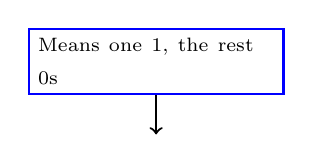
\begin{tikzpicture}
        \draw[->, thick] node[draw, text width=3cm, above, draw=blue] 
             {{\ssmall Means one 1, the rest 0s}}
             (0,0)--++(0, -0.5);
        \end{tikzpicture} 
    \end{center}
    
    \vspace{-20pt}
    
    \item Words can be represented by \textcolor{blue}{one-hot} vectors
    
    \begin{align*}
        \text { motel } &= [0\,0\,0\,0\,0\,0\,0\,0\,1\,0\,0\,0\,0\,0\,0\,0] \\
        \text { hotel } &= [0\,0\,0\,0\,1\,0\,0\,0\,0\,0\,0\,0\,0\,0\,0\,0]
    \end{align*}

    \item Vector dimension $=$ number of words in vocabulary (e.g. 500,000) 
    \end{itemize}
\end{frame}
%%%%%%%%%%%%%%%%%%%%%%%%
\begin{frame}{Problem with words as discrete symbols}
\begin{itemize}
\setlength{\itemsep}{1.2em}

    \item \textcolor{blue}{Example:} in web search, if user searches for \textcolor{blue}{"Seattle motel"}, we would like to match documents containing \textcolor{blue}{"Seattle hotel"}
    
    \item But:
    \vspace{-5pt}
    \begin{align*}
        \text { motel } &= [0\,0\,0\,0\,0\,0\,0\,0\,1\,0\,0\,0\,0\,0\,0\,0] \\
        \text { hotel } &= [0\,0\,0\,0\,1\,0\,0\,0\,0\,0\,0\,0\,0\,0\,0\,0]
    \end{align*}
    \item These two vectors are \textcolor{blue}{orthogonal}
    \item There is no natural notion of \textcolor{blue}{similarity} for one-hot vectors
    \item \textcolor{blue}{Solution:}
    \begin{itemize}
    \vspace{5pt}
        \item Encode similarity in the vectors themselves
    \end{itemize}
    \end{itemize}
\end{frame}
%%%%%%%%%%%%%%%%%%%%%%%%
\begin{frame}{Representing words by their context}
\begin{itemize}
\setlength{\itemsep}{1.2em}

    \item \textcolor{blue}{Core idea:} A word's meaning is given by the words that frequently appear close-by
    \begin{itemize}
    \vspace{3pt}
    \setlength{\itemsep}{0.6em}
        \item \textcolor{cyan}{\textit{"You shall know a word by the company it keeps"}} (J.R. Firth 1957)
        \item One of the most successful ideas of modern statistical NLP
    \end{itemize}
    
    \item When a word $w$ appears in a text, its \textcolor{blue}{context} is the set of words that appear nearby (within a fixed-size window)
    \item Use the many contexts of $w$ to build up a representation of $w$

        
\begin{adjustwidth*}{1em}{-1em}
 \setlength\tabcolsep{0.5pt}
\renewcommand{\arraystretch}{0.8}
    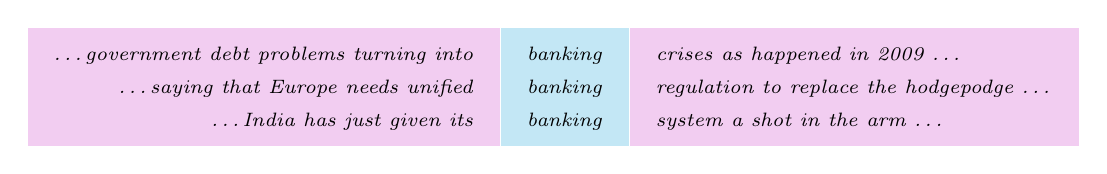
\begin{tikzpicture}[
node distance = 0mm and -0.05mm,% for distance between nodes
   box/.style = {fill}]
\node (n1) [box, fill = Orchid!35] {\begin{tabular}{r}
                  {\ssmall \textit{\dots government debt problems turning into}} \\
                  {\ssmall \textit{\dots saying that Europe needs unified}} \\
                  {\ssmall \textit{\dots India has just given its}} 
                 \end{tabular}};
\node (n2) [box, fill = SkyBlue!50, below right=of n1.north east]
                {\begin{tabular}{c}
                  {\ssmall \textit{banking}}               \\
                  {\ssmall \textit{banking}}               \\
                  {\ssmall \textit{banking}}                
                 \end{tabular}};
 \node (n3) [box, fill = Orchid!35, below right=of n2.north east] {\begin{tabular}{l}
                  {\ssmall \textit{crises as happened in 2009 \dots}} \\
                  {\ssmall \textit{regulation to replace the hodgepodge \dots}} \\
                  {\ssmall \textit{system a shot in the arm \dots}} 
                 \end{tabular}};
    \end{tikzpicture}
\end{adjustwidth*}

  \begin{center}
        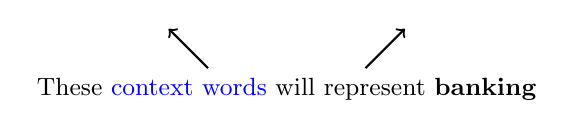
\begin{tikzpicture}
        \node[fill = white , below] at (0,0) 
             {{\small These \textcolor{blue}{context words} will represent \textbf{banking}}};
             \draw[->, thick] (-1,0)--++(-0.5, 0.5);
             \draw[->, thick] (1,0)--++(0.5, 0.5);
        \end{tikzpicture} 
    \end{center}
    
    \end{itemize}
\end{frame}
%%%%%%%%%%%%%%%%%%%%%%%%
\begin{frame}{Word vectors}
\begin{itemize}
\setlength{\itemsep}{1.2em}

    \item We will build a dense vector for each word, chosen so that it is similar to vectors of words that appear in similar contexts
    \vspace{5pt}
    $$
        \text { linguistics = } \quad\left(\begin{array}{r}
        0.286 \\
        0.792 \\
        -0.177 \\
        -0.107 \\
        0.109 \\
        -0.542 \\
        0.349 \\
        0.271
        \end{array}\right)
    $$
    
    \item Note: \textcolor{blue}{word vectors} are sometimes called \textcolor{blue}{word embeddings} or \textcolor{blue}{word representations}
    \end{itemize}
\end{frame}
%%%%%%%%%%%%%%%%%%%%%%%%
\begin{frame}{word2vec: overview}
\begin{itemize}
\setlength{\itemsep}{1.2em}

    \item \textcolor{blue}{word2vec} (Mikolov et al. 2013) is a framework for learning word vectors
    \item \textcolor{blue}{Idea:}
    \begin{itemize}
    \vspace{5pt}
    \setlength{\itemsep}{1.2em}
        \item We have a large corpus of text
        \item Every word in a fixed vocabulary is represented by a vector
        \item Go through each position $t$ in the text, which has a center word $c$ and context ('outside') words $o$
        \item Use the similarity of the word vectors for $c$ and $o$ to \textcolor{blue}{calculate the probability} of $o$ given $c$ (or vice versa)
        \item \textcolor{blue}{Keep adjusting the word vectors} to maximize this probability
    \end{itemize}
    \end{itemize}
\end{frame}
%%%%%%%%%%%%%%%%%%%%%%%%
\begin{frame}{word2vec: overview}
\begin{itemize}
\setlength{\itemsep}{1.2em}

    \item Example windows and process for computing $P(w_{t+j}|w_t)$
    \end{itemize}
    \begin{adjustwidth*}{0em}{2em}
         \setlength\tabcolsep{0.5pt}
        \renewcommand{\arraystretch}{0.8}
            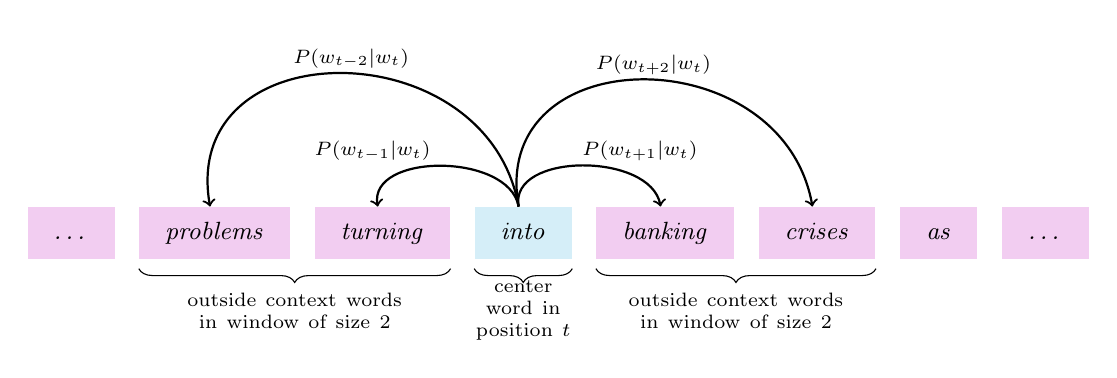
\begin{tikzpicture}[
        node distance = 0mm and 3mm,% for distance between nodes
           box/.style = {fill}]
        \node (n1) [box, fill = Orchid!35] {\begin{tabular}{c}
                          {\small \textit{\dots}}
                         \end{tabular}};
        \node (n2) [box, fill = Orchid!35, below right=of n1.north east] {\begin{tabular}{c}
                          {\small \textit{problems}}
                         \end{tabular}};
        \node (n3) [box, fill = Orchid!35, below right=of n2.north east] {\begin{tabular}{c}
                          {\small \textit{turning}}
                         \end{tabular}};
        \node (n4) [box, fill = SkyBlue!35, below right=of n3.north east] {\begin{tabular}{c}
                          {\small \textit{into}}
                         \end{tabular}};
        \node (n5) [box, fill = Orchid!35, below right=of n4.north east] {\begin{tabular}{c}
                          {\small \textit{banking}}
                         \end{tabular}};
        \node (n6) [box, fill = Orchid!35, below right=of n5.north east] {\begin{tabular}{c}
                          {\small \textit{crises}}
                         \end{tabular}};
        \node (n7) [box, fill = Orchid!35, below right=of n6.north east] {\begin{tabular}{c}
                          {\small \textit{as}}
                         \end{tabular}};
        \node (n8) [box, fill = Orchid!35, below right=of n7.north east] {\begin{tabular}{c}
                          {\small \textit{\dots}}
                         \end{tabular}};
        
        
        \path[->, thick] (n4) edge[loop right,in=100,out=100] node[label={[xshift=0.6cm,yshift=-0.2cm]\ssmall $P(w_{t+1}|w_t)$}]{} (n5);
        \path[->, thick] (n4) edge[loop right,in=100,out=100,looseness = 1.5] node[label={[yshift=-0.2cm]\ssmall $P(w_{t+2}|w_t)$}]{} (n6);
        \path[->, thick] (n4) edge[loop right,in=100,out=100] node[label={[xshift=-1cm,yshift=-0.2cm]\ssmall $P(w_{t-1}|w_t)$}]{} (n3);
        \path[->, thick] (n4) edge[loop right,in=100,out=100,looseness = 1.5] node[label={[yshift=-0.2cm]\ssmall $P(w_{t-2}|w_t)$}]{} (n2);
        
        
        \draw [decorate,decoration={brace,amplitude=5pt,mirror,raise=3ex}]
          (n2.west) -- (n3.east) node[midway, align=center,text width=3cm, yshift=-2.8em]{\baselineskip=1pt \ssmall outside context words in window of size 2 \par};
        \draw [decorate,decoration={brace,amplitude=5pt,mirror,raise=3ex}]
          (n5.west) -- (n6.east) node[midway, align=center,text width=3cm, yshift=-2.8em]{\baselineskip=1pt \ssmall outside context words in window of size 2 \par};
        \draw [decorate,decoration={brace,amplitude=5pt,raise=3ex}]
          (n4.east) -- (n4.west) node[midway, align=center,text width=1.5cm, yshift=-2.8em]{\baselineskip=1pt \ssmall center word in position $t$ \par};
            \end{tikzpicture}
    \end{adjustwidth*}
\end{frame}
%%%%%%%%%%%%%%%%%%%%%%%%
%%%%%%%%%%%%%%%%%%%%%%%%
\begin{frame}{word2vec: overview}
\begin{itemize}
\setlength{\itemsep}{1.2em}

    \item Example windows and process for computing $P(w_{t+j}|w_t)$
    \end{itemize}
    \begin{adjustwidth*}{0em}{0em}
         \setlength\tabcolsep{0.5pt}
        \renewcommand{\arraystretch}{0.8}
            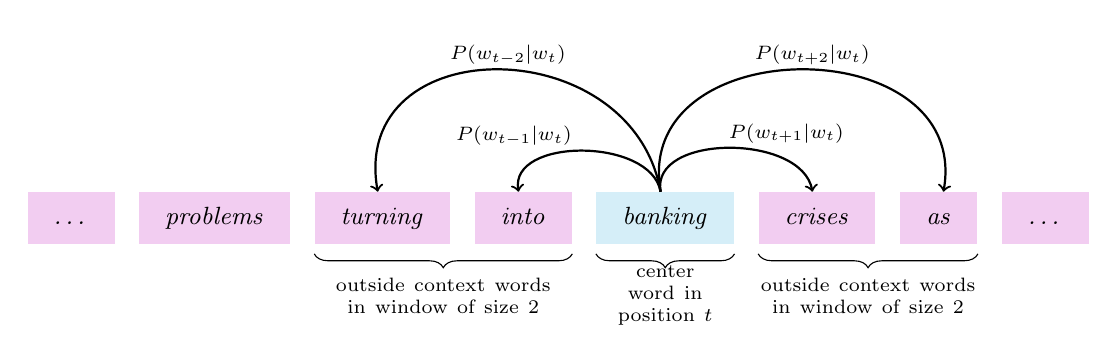
\begin{tikzpicture}[
        node distance = 0mm and 3mm,% for distance between nodes
           box/.style = {fill}]
        \node (n1) [box, fill = Orchid!35] {\begin{tabular}{c}
                          {\small \textit{\dots}}
                         \end{tabular}};
        \node (n2) [box, fill = Orchid!35, below right=of n1.north east] {\begin{tabular}{c}
                          {\small \textit{problems}}
                         \end{tabular}};
        \node (n3) [box, fill = Orchid!35, below right=of n2.north east] {\begin{tabular}{c}
                          {\small \textit{turning}}
                         \end{tabular}};
        \node (n4) [box, fill = Orchid!35, below right=of n3.north east] {\begin{tabular}{c}
                          {\small \textit{into}}
                         \end{tabular}};
        \node (n5) [box, fill = SkyBlue!35, below right=of n4.north east] {\begin{tabular}{c}
                          {\small \textit{banking}}
                         \end{tabular}};
        \node (n6) [box, fill = Orchid!35, below right=of n5.north east] {\begin{tabular}{c}
                          {\small \textit{crises}}
                         \end{tabular}};
        \node (n7) [box, fill = Orchid!35, below right=of n6.north east] {\begin{tabular}{c}
                          {\small \textit{as}}
                         \end{tabular}};
        \node (n8) [box, fill = Orchid!35, below right=of n7.north east] {\begin{tabular}{c}
                          {\small \textit{\dots}}
                         \end{tabular}};
        
        
        \path[->, thick] (n5) edge[loop right,in=100,out=100] node[label={[xshift=0.6cm,yshift=-0.2cm]\ssmall $P(w_{t+1}|w_t)$}]{} (n6);
        \path[->, thick] (n5) edge[loop right,in=80,out=100,looseness = 1.5] node[label={[yshift=-0.2cm]\ssmall $P(w_{t+2}|w_t)$}]{} (n7);
        \path[->, thick] (n5) edge[loop right,in=100,out=100] node[label={[xshift=-1cm,yshift=-0.2cm]\ssmall $P(w_{t-1}|w_t)$}]{} (n4);
        \path[->, thick] (n5) edge[loop right,in=100,out=100,looseness = 1.5] node[label={[yshift=-0.2cm]\ssmall $P(w_{t-2}|w_t)$}]{} (n3);
        
        
        \draw [decorate,decoration={brace,amplitude=5pt,mirror,raise=3ex}]
          (n3.west) -- (n4.east) node[midway, align=center,text width=3cm, yshift=-2.8em]{\baselineskip=1pt \ssmall outside context words in window of size 2 \par};
        \draw [decorate,decoration={brace,amplitude=5pt,mirror,raise=3ex}]
          (n6.west) -- (n7.east) node[midway, align=center,text width=3cm, yshift=-2.8em]{\baselineskip=1pt \ssmall outside context words in window of size 2 \par};
        \draw [decorate,decoration={brace,amplitude=5pt,raise=3ex}]
          (n5.east) -- (n5.west) node[midway, align=center,text width=1.45cm, yshift=-2.8em]{\baselineskip=1pt \ssmall center word in position $t$ \par};
    \end{tikzpicture}
\end{adjustwidth*}
\end{frame}
%%%%%%%%%%%%%%%%%%%%%%%%
\begin{frame}{word2vec: objective function}
\begin{itemize}
\setlength{\itemsep}{1.2em}
    \item For each position $t = 1,\dots,T$, predict context words within a window of fixed size $m$, given center word $w_j$
    $$
        L(\theta)=\prod_{t=1}^{T} \prod_{-m \leq j \leq m} P\left(w_{t+j} \mid w_{t} ; \theta\right)
    $$
    \begin{itemize}
    \setlength{\itemsep}{1.2em}
        \item $\theta$ is all the variables to be optimized
    \end{itemize}
    \item The \textcolor{blue}{objective function} $J(\theta)$ is the average negative log likelihood:
    $$
    J(\theta)=-\frac{1}{T} \log L(\theta)=-\frac{1}{T} \sum_{t=1}^{T} \sum_{m \leq j \leq m} \log P\left(w_{t+j} \mid w_{t} ; \theta\right)
    $$
    \begin{itemize}
    \setlength{\itemsep}{1.2em}
        \item Minimizing objective function $\Leftrightarrow$ Maximizing predictive accuracy
    \end{itemize}
    \end{itemize}
\end{frame}
%%%%%%%%%%%%%%%%%%%%%%%%
\begin{frame}{word2vec: objective function}
\begin{itemize}
\setlength{\itemsep}{1.2em}
    \item We want to minimize the objective function
    $$
    J(\theta)=-\frac{1}{T} \sum_{t=1}^{T} \sum_{m \leq j \leq m} \log P\left(w_{t+j} \mid w_{t} ; \theta\right)
    $$
    \item \textcolor{blue}{Question:} How to calculate $P\left(w_{t+j} \mid w_{t};\theta\right)$
    \item \textcolor{blue}{Answer:} We will use two vectors per word $w$:
    \begin{itemize}
    \setlength{\itemsep}{0.8em}
    \vspace{5pt}
        \item $v_w$ when $w$ is a center word
        \item $u_w$ when $w$ is a context word
    \end{itemize}
    \item Then for a center word $c$ and a context word $o$:
    $$
    P(o \mid c)=\frac{\exp \left(u_{o}^{T} v_{c}\right)}{\sum_{w \in V} \exp \left(u_{w}^{T} v_{c}\right)}
    $$
    \end{itemize}
\end{frame}
%%%%%%%%%%%%%%%%%%%%%%%%
\begin{frame}{word2vec: overview with vectors}
\begin{itemize}
\setlength{\itemsep}{1.2em}
    \item Example windows and process for computing $P(w_{t+j}\mid w_t)$
    \item $P(u_{problems}\mid v_{into})$ is short for \textcolor{blue}{$P(problems|into,u_{problems},v_{into},\theta)$}
    \vspace{10pt}
    \begin{adjustwidth*}{0em}{2em}
         \setlength\tabcolsep{0.5pt}
        \renewcommand{\arraystretch}{0.8}
            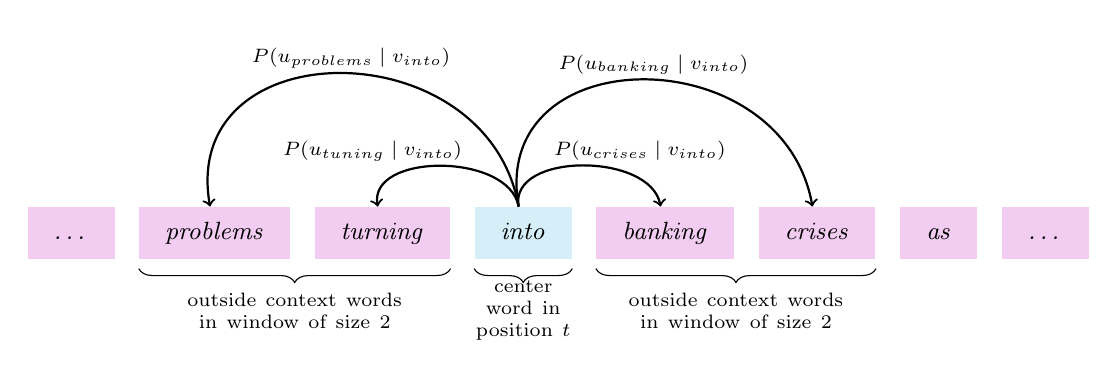
\begin{tikzpicture}[
        node distance = 0mm and 3mm,% for distance between nodes
           box/.style = {fill}]
        \node (n1) [box, fill = Orchid!35] {\begin{tabular}{c}
                          {\small \textit{\dots}}
                         \end{tabular}};
        \node (n2) [box, fill = Orchid!35, below right=of n1.north east] {\begin{tabular}{c}
                          {\small \textit{problems}}
                         \end{tabular}};
        \node (n3) [box, fill = Orchid!35, below right=of n2.north east] {\begin{tabular}{c}
                          {\small \textit{turning}}
                         \end{tabular}};
        \node (n4) [box, fill = SkyBlue!35, below right=of n3.north east] {\begin{tabular}{c}
                          {\small \textit{into}}
                         \end{tabular}};
        \node (n5) [box, fill = Orchid!35, below right=of n4.north east] {\begin{tabular}{c}
                          {\small \textit{banking}}
                         \end{tabular}};
        \node (n6) [box, fill = Orchid!35, below right=of n5.north east] {\begin{tabular}{c}
                          {\small \textit{crises}}
                         \end{tabular}};
        \node (n7) [box, fill = Orchid!35, below right=of n6.north east] {\begin{tabular}{c}
                          {\small \textit{as}}
                         \end{tabular}};
        \node (n8) [box, fill = Orchid!35, below right=of n7.north east] {\begin{tabular}{c}
                          {\small \textit{\dots}}
                         \end{tabular}};
        
        
        \path[->, thick] (n4) edge[loop right,in=100,out=100] node[label={[xshift=0.6cm,yshift=-0.2cm]\ssmall $P(u_{crises}\mid v_{into})$}]{} (n5);
        \path[->, thick] (n4) edge[loop right,in=100,out=100,looseness = 1.5] node[label={[yshift=-0.2cm]\ssmall $P(u_{banking}\mid v_{into})$}]{} (n6);
        \path[->, thick] (n4) edge[loop right,in=100,out=100] node[label={[xshift=-1cm,yshift=-.2cm]\ssmall $P(u_{tuning}\mid v_{into})$}]{} (n3);
        \path[->, thick] (n4) edge[loop right,in=100,out=100,looseness = 1.5] node[label={[yshift=-0.2cm]\ssmall $P(u_{problems}\mid v_{into})$}]{} (n2);
        
        
        \draw [decorate,decoration={brace,amplitude=5pt,mirror,raise=3ex}]
          (n2.west) -- (n3.east) node[midway, align=center,text width=3cm, yshift=-2.8em]{\baselineskip=1pt \ssmall outside context words in window of size 2 \par};
        \draw [decorate,decoration={brace,amplitude=5pt,mirror,raise=3ex}]
          (n5.west) -- (n6.east) node[midway, align=center,text width=3cm, yshift=-2.8em]{\baselineskip=1pt \ssmall outside context words in window of size 2 \par};
        \draw [decorate,decoration={brace,amplitude=5pt,raise=3ex}]
          (n4.east) -- (n4.west) node[midway, align=center,text width=1.5cm, yshift=-2.8em]{\baselineskip=1pt \ssmall center word in position $t$ \par};
            \end{tikzpicture}
    \end{adjustwidth*}
    \end{itemize}
\end{frame}
%%%%%%%%%%%%%%%%%%%%%%%%
\begin{frame}{word2vec: overview with vectors}
\begin{itemize}
\setlength{\itemsep}{1.2em}
    \item Example windows and process for computing $P(w_{t+j}\mid w_t)$
    \begin{adjustwidth*}{0em}{0em}
         \setlength\tabcolsep{0.5pt}
        \renewcommand{\arraystretch}{0.8}
            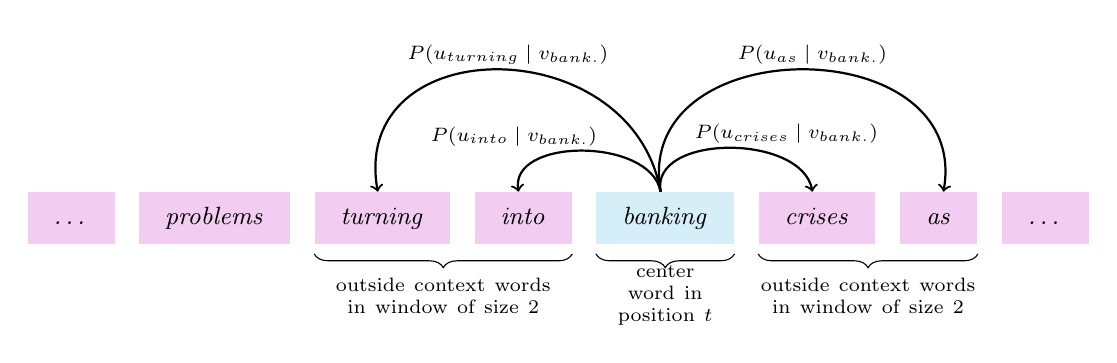
\begin{tikzpicture}[
        node distance = 0mm and 3mm,% for distance between nodes
           box/.style = {fill}]
        \node (n1) [box, fill = Orchid!35] {\begin{tabular}{c}
                          {\small \textit{\dots}}
                         \end{tabular}};
        \node (n2) [box, fill = Orchid!35, below right=of n1.north east] {\begin{tabular}{c}
                          {\small \textit{problems}}
                         \end{tabular}};
        \node (n3) [box, fill = Orchid!35, below right=of n2.north east] {\begin{tabular}{c}
                          {\small \textit{turning}}
                         \end{tabular}};
        \node (n4) [box, fill = Orchid!35, below right=of n3.north east] {\begin{tabular}{c}
                          {\small \textit{into}}
                         \end{tabular}};
        \node (n5) [box, fill = SkyBlue!35, below right=of n4.north east] {\begin{tabular}{c}
                          {\small \textit{banking}}
                         \end{tabular}};
        \node (n6) [box, fill = Orchid!35, below right=of n5.north east] {\begin{tabular}{c}
                          {\small \textit{crises}}
                         \end{tabular}};
        \node (n7) [box, fill = Orchid!35, below right=of n6.north east] {\begin{tabular}{c}
                          {\small \textit{as}}
                         \end{tabular}};
        \node (n8) [box, fill = Orchid!35, below right=of n7.north east] {\begin{tabular}{c}
                          {\small \textit{\dots}}
                         \end{tabular}};
        
        
        \path[->, thick] (n5) edge[loop right,in=100,out=100] node[label={[xshift=0.6cm,yshift=-0.2cm]\ssmall $P(u_{crises}\mid v_{bank.})$}]{} (n6);
        \path[->, thick] (n5) edge[loop right,in=80,out=100,looseness = 1.5] node[label={[yshift=-0.2cm]\ssmall $P(u_{as}\mid v_{bank.})$}]{} (n7);
        \path[->, thick] (n5) edge[loop right,in=100,out=100] node[label={[xshift=-1cm,yshift=-0.2cm]\ssmall $P(u_{into}\mid v_{bank.})$}]{} (n4);
        \path[->, thick] (n5) edge[loop right,in=100,out=100,looseness = 1.5] node[label={[yshift=-0.2cm]\ssmall $P(u_{turning}\mid v_{bank.})$}]{} (n3);
        
        
        \draw [decorate,decoration={brace,amplitude=5pt,mirror,raise=3ex}]
          (n3.west) -- (n4.east) node[midway, align=center,text width=3cm, yshift=-2.8em]{\baselineskip=1pt \ssmall outside context words in window of size 2 \par};
        \draw [decorate,decoration={brace,amplitude=5pt,mirror,raise=3ex}]
          (n6.west) -- (n7.east) node[midway, align=center,text width=3cm, yshift=-2.8em]{\baselineskip=1pt \ssmall outside context words in window of size 2 \par};
        \draw [decorate,decoration={brace,amplitude=5pt,raise=3ex}]
          (n5.east) -- (n5.west) node[midway, align=center,text width=1.45cm, yshift=-2.8em]{\baselineskip=1pt \ssmall center word in position $t$ \par};
    \end{tikzpicture}
\end{adjustwidth*}    
\end{itemize}
\end{frame}
%%%%%%%%%%%%%%%%%%%%%%%%
\begin{frame}{word2vec: prediction function}
        $$
        P(o \mid c)=\frac{\exp \left(\textcolor{orange}{u_{o}^{T} v_{c}}\right)}{\textcolor{blue}{\sum_{w \in V} \exp \left(u_{w}^{T} v_{c}\right)}}
        $$
    \begin{itemize}
        \setlength{\itemsep}{1em}

        \item \textcolor{orange}{$u_{o}^{T} v_{c}$}: dot product compares similarity of $o$ and $c$. Larger dot product implies a larger probability
        \item \textcolor{blue}{$\sum_{w \in V} \exp \left(u_{w}^{T} v_{c}\right)$}: after taking exponent, normalize over entire vocabulary

        \item This is an example of the \textcolor{blue}{softmax function} $\mathbb{R}^n \rightarrow \mathbb{R}^n$
        \item The softmax function maps arbitrary values $x_i$ to a probability distribution $p_i$
        \begin{itemize}
            \setlength{\itemsep}{0.8em}
            \vspace{5pt}
            \item \textcolor{blue}{"max"} because amplifies probability of largest $x_i$
            \item \textcolor{blue}{"soft"} because still assigns some probability to smaller $x_i$
        \end{itemize}
    \end{itemize}
\end{frame}
%%%%%%%%%%%%%%%%%%%%%%%%
\begin{frame}{To train the model: compute all vector gradients}

    \begin{itemize}
        \setlength{\itemsep}{1em}
        
        \item \textcolor{blue}{Recall}: $\theta$ represents all model parameters, in one long vector
        \item In our case with $d$-dimensional vectors and $V$-many words:
        $$
        \theta=\left[\begin{array}{l}
        v_{aardvark} \\
        v_{a} \\
        \vdots \\
        v_{zebra} \\
        u_{aardvark} \\
        u_{a} \\
        \vdots \\
        u_{zebra}
        \end{array}\right] \in \mathbb{R}^{2 d V}
        $$
        \item \textcolor{blue}{Recall}: every word has two vectors
        \item We then optimize these parameters using \textcolor{blue}{stochastic gradient descent}
    \end{itemize}
    
\end{frame}
%%%%%%%%%%%%%%%%%%%%%%%%
\begin{frame}{word2vec: gradient descent}
    \begin{itemize}
        \setlength{\itemsep}{1em}
        \item We have a cost function $J(\theta)$ we want to minimize
        \item \textcolor{blue}{Idea}: for the current value of $\theta$, calculate the gradient of $J(\theta)$, then take a small step in the direction of the negative gradient. Repeat. 
        \begin{center}
        \vspace{5pt}
    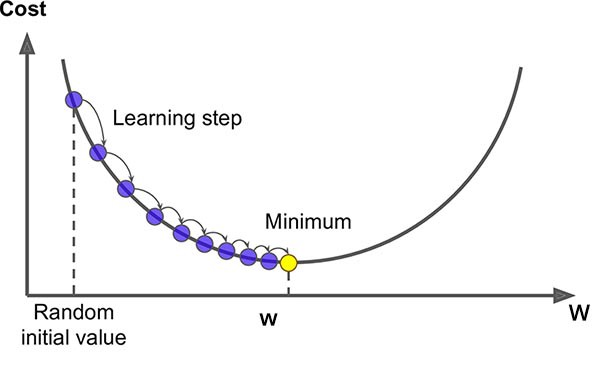
\includegraphics[scale=0.4]{Images/we_gradient.jpeg}
    \end{center}
    \end{itemize}
    
\end{frame}
%%%%%%%%%%%%%%%%%%%%%%%%
\begin{frame}{word2vec: stochastic gradient descent}
    \begin{itemize}
        \setlength{\itemsep}{1em}
        \item \textcolor{blue}{Problem}: $J(\theta)$ is a function of \textcolor{blue}{all} windows in the corpus
        \begin{itemize}
        \vspace{5pt}
            \item $\nabla_{\theta}J(\theta)$ may be very expensive to compute
        \end{itemize}
        \item You would wait a very long time before making a single update. A very bad idea for pretty much all neural nets
        \item \textcolor{blue}{Solution}: stochastic gradient descent (SGD)
        \begin{itemize}
        \vspace{5pt}
            \item Repeatedly sample windows, and update after each one
        \end{itemize}
                \begin{center}
        \vspace{5pt}
    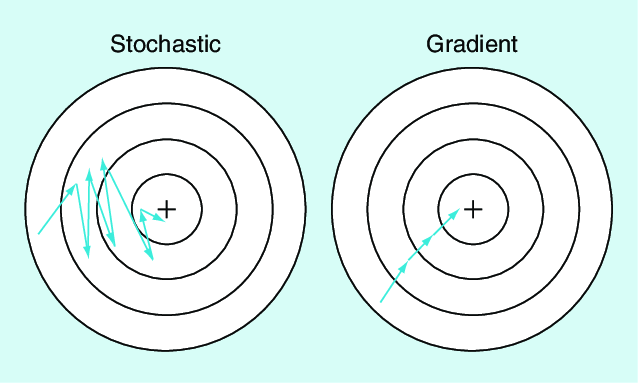
\includegraphics[scale=0.25]{Images/we_SGD.png}
    \end{center}
    \end{itemize}
    
\end{frame}
%%%%%%%%%%%%%%%%%%%%%%%%
\begin{frame}{word2vec: applications}

    \begin{itemize}
        \setlength{\itemsep}{1em}
        
        \item Once the vectors are constructed, they can be used to represent relations between words
        \begin{center}
    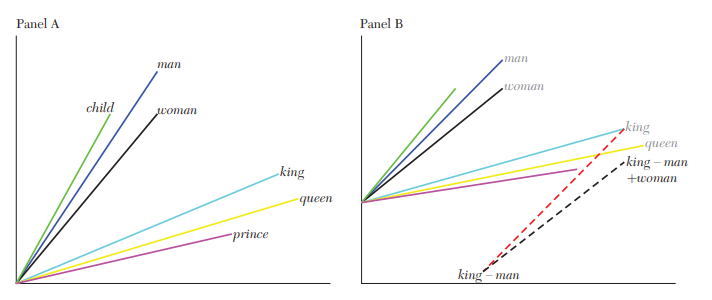
\includegraphics[scale=0.6]{Images/we_gentzkow.png}
    \end{center}
    \end{itemize}
    
\end{frame}
%%%%%%%%%%%%%%%%%%%%%%%%
\begin{frame}{Garg, Schiebinger, Jurafsky, and Zou (2018)}
\begin{itemize}
\setlength{\itemsep}{1.2em}
    \item \textcolor{blue}{Goal}: develop a systematic framework to analyze word embeddings trained over a century of text data to identify historical patterns of bias and stereotype changes in the US
    \item \textcolor{blue}{Motivation}: in word-embedding models, words are assigned to a high-dimensional vector in a way that they capture relationships not found through simple co-occurrence analysis
    \item \textcolor{blue}{Idea}: exploit differences in Euclidean distance between ethnic-gender terms and professions-stereotypes words to quantify historical trends
    \item \textcolor{blue}{Main findings}: the embedding captures societal shifts and sheds light on how specific adjectives and occupations became more closely associated with certain populations over time
\end{itemize}
\end{frame}
%%%%%%%%%%%%%%%%%%%%%%%%
\begin{frame}{GSJZ (2018): data}
\begin{itemize}
\setlength{\itemsep}{1.2em}
    \item Word embeddings:
    \begin{itemize}
    \setlength{\itemsep}{1.2em}
    \vspace{5pt}
        \item word2vec embeddings trained on the Google News dataset
        \item Nine decade-specific embeddings trained on text from the Corpus of Historical American English
    \end{itemize}
    \item Word lists: 
    \begin{itemize}
        \setlength{\itemsep}{1.2em}
        \vspace{5pt}
        \item Gender: \textit{he, she, son, daughter, male, female, boy, girl, etc.}
        \item Ethniticty: \textit{harris, ruiz, cho, thompson, gomez, lin, etc.}
        \item Occupations: \textit{janitor, teacher, shoemaker, scientist, carpenter, etc.}
        \item Adjectives: \textit{headstrong, inventive, enterprising, poised, moody, etc.}
    \end{itemize}
\end{itemize}
\end{frame}
%%%%%%%%%%%%%%%%%%%%%%%%
\begin{frame}{GSJZ (2018): methodology}
\begin{itemize}
    \setlength{\itemsep}{1.2em}
    \vspace{5pt}
    \item Measure the strength of association between occupations or adjectives (neutral words) and a gender or ethnicity
    \begin{enumerate}
        \setlength{\itemsep}{0.8em}
    \vspace{5pt}
        \item Compute the average vector representation of a gender or ethnic group
        \item Calculate the average Euclidean distance between the representative vector and each vector in a list of neutral words
        \item Use the difference of the average distance between gender or ethnicity pairs as a measure of embedding bias
    \end{enumerate}
    \item e.g. the occupational embedding bias for women
    \begin{enumerate}
        \setlength{\itemsep}{0.8em}
    \vspace{5pt}
        \item Compute average embedding distance between words \textit{she, female} and occupational words \textit{teacher, lawyer}. Repeat for words {he, male}
        \item Compute the difference in average distances between group pair
        $$
        \text { relative norm distance }=\sum_{v_{m} \in M}\left\|v_{m}-v_{1}\right\|_{2}-\left\|v_{m}-v_{2}\right\|_{2}
        $$
    \end{enumerate}
\end{itemize}
\end{frame}
%%%%%%%%%%%%%%%%%%%%%%%%
\begin{frame}{GSJZ (2018): gender bias snapshot validation}
\begin{figure}
    \centering
    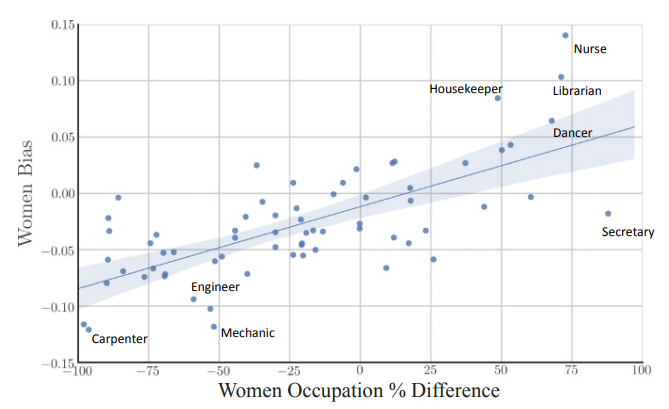
\includegraphics[scale = 0.5]{Images/gsjz_validation1.png}
    \end{figure}
    \begin{itemize}
        \item {\small Occupation difference as the relative percentage of women in each occupation using data from the Integrated Public Use Microdata Series}
    \end{itemize}
\end{frame}
%%%%%%%%%%%%%%%%%%%%%%%%
\begin{frame}{GSJZ (2018): gender bias historical validation}
\begin{figure}
    \centering
    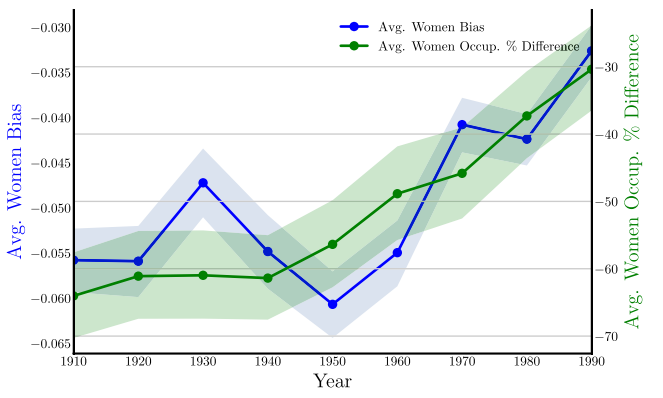
\includegraphics[scale = 0.6]{Images/gsjz_validation2.png}
\end{figure}
\end{frame}
%%%%%%%%%%%%%%%%%%%%%%%%
\begin{frame}{GSJZ (2018): ethnic bias historical validation}
\begin{figure}
    \centering
    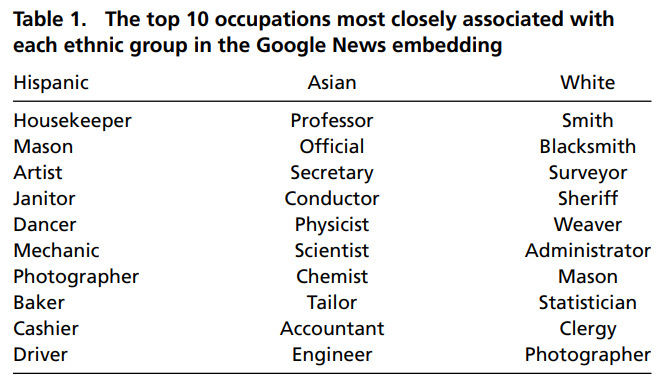
\includegraphics[scale = 0.5]{Images/gsjz_validation3.png}
\end{figure}
\end{frame}
%%%%%%%%%%%%%%%%%%%%%%%%
\begin{frame}{GSJZ (2018): ethnic bias historical validation}
\begin{figure}
    \centering
    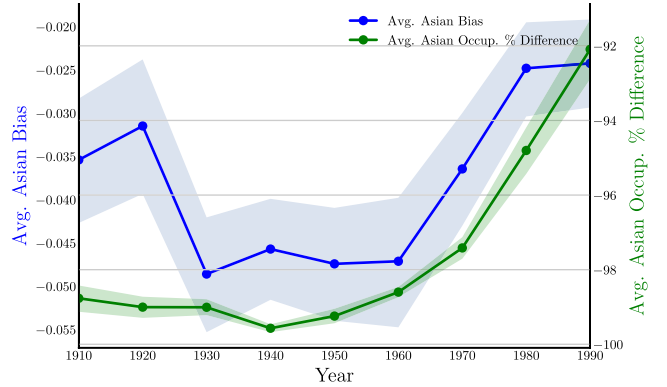
\includegraphics[scale = 0.6]{Images/gsjz_validation4.png}
\end{figure}
\end{frame}
%%%%%%%%%%%%%%%%%%%%%%%%
\begin{frame}{GSJZ (2018): quantifying gender stereotypes}
\begin{figure}
    \centering
    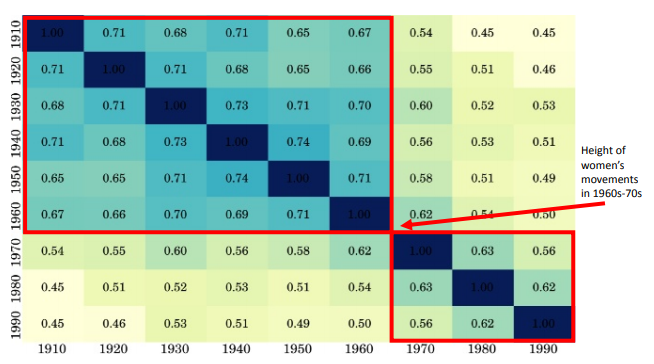
\includegraphics[scale = 0.6]{Images/gsjz_quantify1.png}
\end{figure}
\begin{itemize}
    \item {\small Pearson correlation in embedding bias scores for adjectives over time}
\end{itemize}
\end{frame}
%%%%%%%%%%%%%%%%%%%%%%%%
\begin{frame}{GSJZ (2018): quantifying gender stereotypes}
\begin{figure}
    \centering
    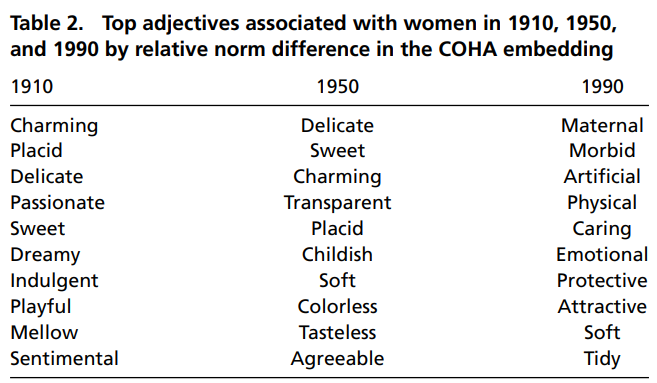
\includegraphics[scale = 0.5]{Images/gsjz_quantify2.png}
\end{figure}
\end{frame}
%%%%%%%%%%%%%%%%%%%%%%%%
\begin{frame}{GSJZ (2018): quantifying ethnic stereotypes}
\begin{figure}
    \centering
    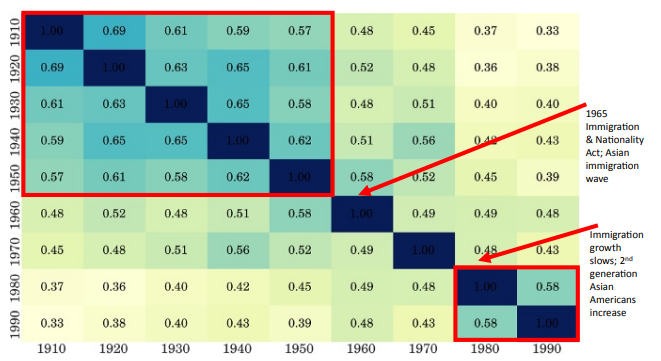
\includegraphics[scale = 0.6]{Images/gsjz_quantify3.png}
\end{figure}
\begin{itemize}
    \item {\small Pearson correlation in embedding Asian bias scores for adjectives}
\end{itemize}
\end{frame}
%%%%%%%%%%%%%%%%%%%%%%%%
\begin{frame}{GSJZ (2018): quantifying ethnic stereotypes}
\begin{figure}
    \centering
    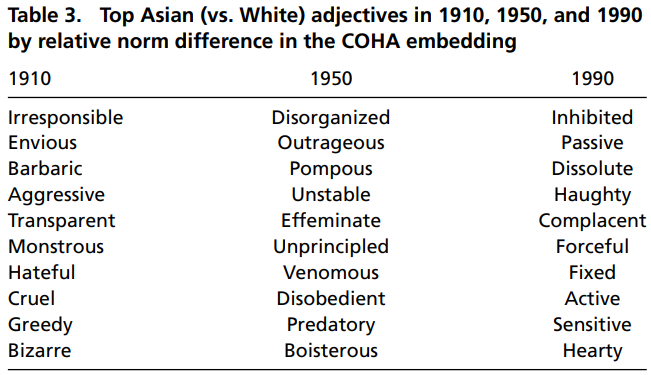
\includegraphics[scale = 0.5]{Images/gsjz_quantify4.png}
\end{figure}
\end{frame}
%%%%%%%%%%%%%%%%%%%%%%%%
\begin{frame}{GSJZ (2018): quantifying ethnic stereotypes}
\begin{figure}
    \centering
    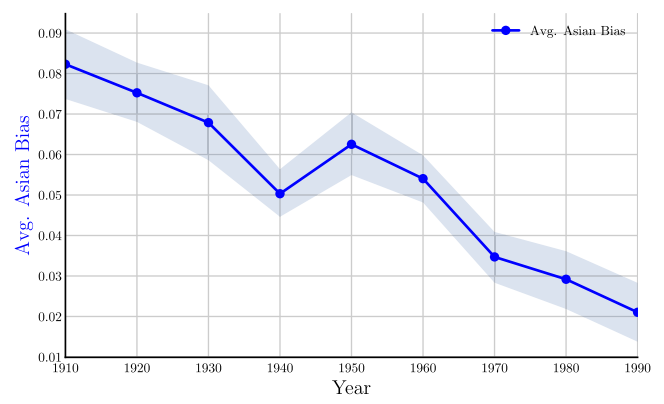
\includegraphics[scale = 0.6]{Images/gsjz_quantify5.png}
\end{figure}
\begin{itemize}
    \item {\small Asian bias score over time for words related to outsiders in COHA data}
\end{itemize}
\end{frame}
%%%%%%%%%%%%%%%%%%%%%%%%
\begin{frame}{Kozlowski, Taddy and Evans (2019): geometry of culture}

    \begin{itemize}
    \setlength{\itemsep}{0.8em}
        \item \textcolor{blue}{Motivation}
        \begin{itemize}
        \setlength{\itemsep}{0.8em}
            \item If text represents culture, can we construct \textcolor{blue}{cultural dimensions} of class from the dimension of word embedding vectors?
            \item Has the \textcolor{blue}{meaning} of these dimensions changed over the XXth century?
        \end{itemize}
        \item Class as the systematic and hierarchical distinction of people and groups in social standing. Dimension-specific nuances:
        \begin{itemize}
        \setlength{\itemsep}{0.8em}
\vspace{5pt}
            \item \textbf{Money:} easy to convert into various forms of power $\rightarrow$ \textcolor{blue}{affluence} 
            \item \textbf{Education:} determines the labor market position $\rightarrow$ \textcolor{blue}{education} 
            \item \textbf{Status:} based on authority and social position $\rightarrow$ \textcolor{blue}{status} 
            \item \textbf{Cultivated taste:} based on the culture consumed $\rightarrow$ \textcolor{blue}{cultivation} 
            \item \textbf{Gender:} misogynistic or patriarchal hierarchies $\rightarrow$ \textcolor{blue}{gender} 
            \item \textbf{Race:} reflected in post-colonial, structural racism $\rightarrow$ \textcolor{blue}{race} 
        \end{itemize}
        
    \end{itemize}
    
\end{frame}
%%%%%%%%%%%%%%%%%%%%%%%%
\begin{frame}{KTE (2019): the cultural dimensions of class}
    \begin{itemize}
    \setlength{\itemsep}{1.5em}
        \item These dimensions can be represented through semantic contrasts
        \begin{itemize}
        \setlength{\itemsep}{0.8em}
\vspace{10pt}
            \item \textbf{Affluence:} rich vs poor, wealthy vs impoverished, luxury vs cheap
            \item \textbf{Education:} educated vs uneducated, knowledgeable vs ignorant
            \item \textbf{Status:} acclaimed vs modest, eminent vs mundane 
            \item \textbf{Cultivation:} civil vs uncivil, cultured vs uncultured
            \item \textbf{Gender:} masculine vs feminine, he vs she, male vs female
            \item \textbf{Race:} black vs white, African vs European
        \end{itemize}
        \item \textcolor{blue}{Main idea:} words that are opposites semantically will display systematic differences in their vector representation
    \end{itemize}
\end{frame}
%%%%%%%%%%%%%%%%%%%%%%%%
\begin{frame}{KTE (2019): the cultural dimensions of class}
    \begin{itemize}
    \setlength{\itemsep}{1.5em}
        \item \textcolor{blue}{Intuition:} solving an analogy is equivalent to projecting a word vector onto a specific dimension
$$\overrightarrow{\text {king}}+\overrightarrow{\text {woman}}-\overrightarrow{\operatorname{man}} \approx \overrightarrow{\text {queen}}$$
	\item {\small The projection of the word vector for king onto a gender dimension captured by $\overrightarrow{\text {woman}}-\overrightarrow{\operatorname{man}}$ yields the word vector for queen}
	\item Collate lists of antonyms similar to $\overrightarrow{\text {woman}}-\overrightarrow{\operatorname{man}}$ for the different dimensions of class, i.e. $\overrightarrow{\text {rich}}-\overrightarrow{\operatorname{poor}}$
	\item Project words onto dimension-specific antonym lists to identify the cultural associations embedded in the word
$$\overrightarrow{\text {hockey}}+\overrightarrow{\text {rich}}-\overrightarrow{\operatorname{poor}} \approx \overrightarrow{\text {lacrosse}}$$
    \end{itemize}
\end{frame}
%%%%%%%%%%%%%%%%%%%%%%%%
\begin{frame}{KTE (2019): the cultural dimensions of class}
\begin{figure}
    \centering
    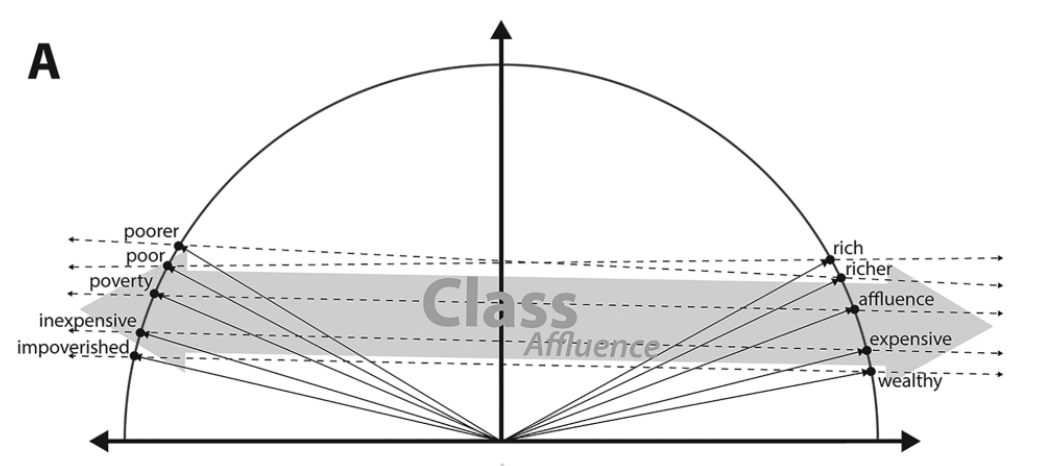
\includegraphics[scale = 0.4]{Images/kte_class_affluence.png}
    \end{figure}
\end{frame}
%%%%%%%%%%%%%%%%%%%%%%%%
\begin{frame}{KTE (2019): the cultural dimensions of class}
\begin{figure}
    \centering
    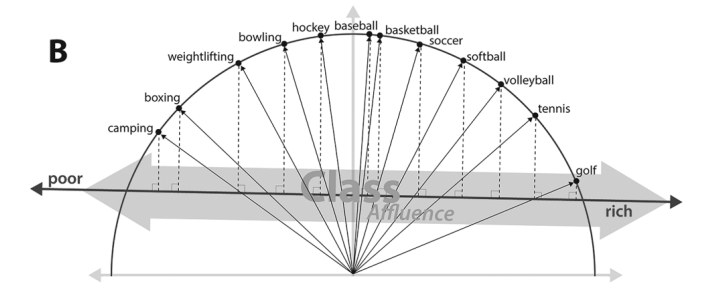
\includegraphics[scale = 0.6]{Images/kte_class_sports.png}
    \end{figure}
\end{frame}
%%%%%%%%%%%%%%%%%%%%%%%%
\begin{frame}{KTE (2019): the cultural dimensions of class}
\begin{figure}
    \centering
    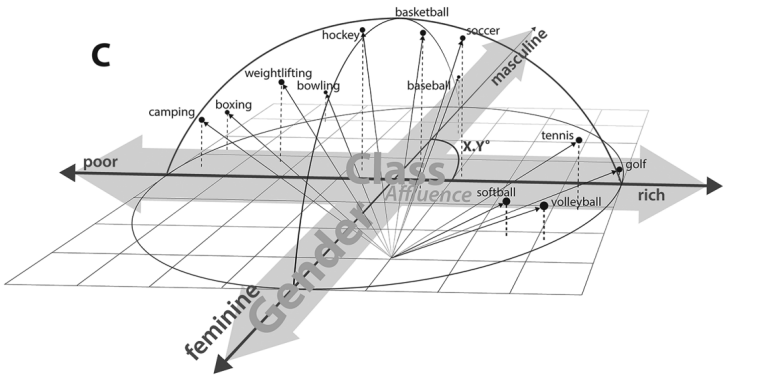
\includegraphics[scale = 0.55]{Images/kte_class_gender_sports.png}
    \end{figure}
\end{frame}
%%%%%%%%%%%%%%%%%%%%%%%%
\begin{frame}{KTE (2019): data and methods}
    \begin{itemize}
    \setlength{\itemsep}{1.2em}
        \item Use three pre-trained \textcolor{blue}{word embedding} models:
        \begin{itemize}
        \setlength{\itemsep}{0.8em}
\vspace{5pt}
            \item Google Ngrams US
            \item Google News embeddings
            \item GloVe embeddings
        \end{itemize}
        \item Trained via Google Ngram corpus
            \begin{itemize}
            \setlength{\itemsep}{0.8em}
    \vspace{5pt}
                \item 6\% of all books ever published
                \item Only look at 5-grams
                \item Divide corpus by decades
                \item Keep only words that appear $>$ 25 times
        \end{itemize}
	\item Antonym lists compiled from five thesauri
    \end{itemize}
\end{frame}
%%%%%%%%%%%%%%%%%%%%%%%%
\begin{frame}{KTE (2019): data}
\begin{figure}
    \centering
    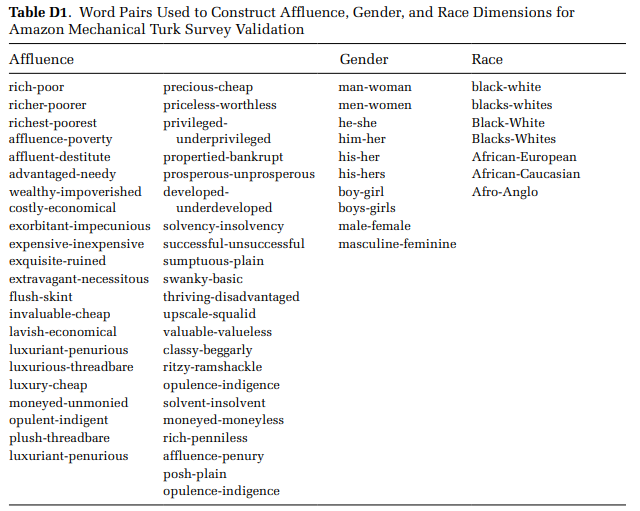
\includegraphics[scale = 0.5]{Images/kte_methods1.png}
    \end{figure}
\end{frame}
%%%%%%%%%%%%%%%%%%%%%%%%
\begin{frame}{KTE (2019): data}
\begin{figure}
    \centering
    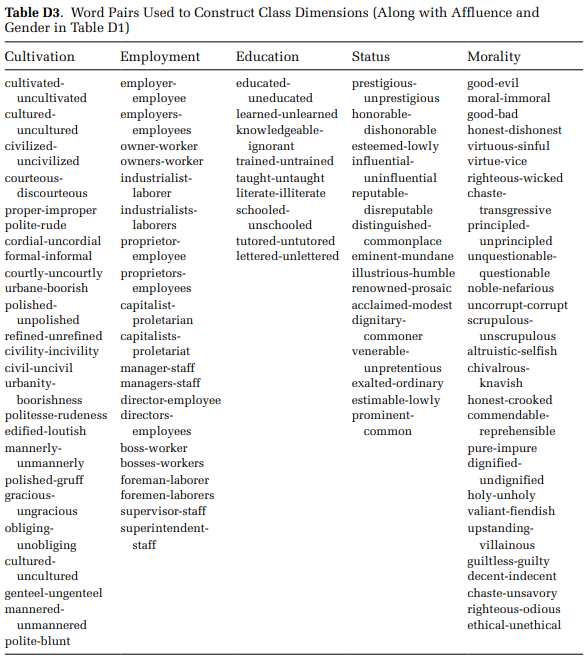
\includegraphics[scale = 0.5]{Images/kte_methods2.png}
    \end{figure}
\end{frame}
%%%%%%%%%%%%%%%%%%%%%%%%
\begin{frame}{KTE (2019): methods}
    \begin{itemize}
    \setlength{\itemsep}{1.5em}
        \item For each class dimension, calculate the following:
$$
\frac{\sum_{p}^{|P|} \overrightarrow{p_{1}}-\overrightarrow{p_{2}}}{|P|}
$$

        \item $p$ are all antonym couples in set $P$ of relevant words by context 
        \item The projection of a word vector onto a dimension is computed using cosine similarity

    \end{itemize}
\end{frame}
%%%%%%%%%%%%%%%%%%%%%%%%
\begin{frame}{KTE (2019): methods}{Validation}
    \begin{itemize}
    \setlength{\itemsep}{1.5em}
        \item Use two surveys
        \begin{itemize}
\vspace{10pt}
        \setlength{\itemsep}{1.2em}
            \item \textbf{Modern Survey:} rate 59 words on different dimensions (class, race, gender)
            \item \textbf{\textit{Historical} Survey:} rate 360 words on 20 semantic dimensions (good/bad, soft/hard, \dots)
        \end{itemize}

        \item Example:
        \begin{itemize}
            \item On a scale from 0 (very working class) to 100 (very upper class), how would you rate a steak?
        \end{itemize}
    \end{itemize}
\begin{figure}
    \centering
    \includegraphics[scale = 0.4]{Images/kte_validationturk.png}
    \end{figure}
\end{frame}
%%%%%%%%%%%%%%%%%%%%%%%%
\begin{frame}{KTE (2019): methods}{Validation}
\begin{figure}
    \centering
    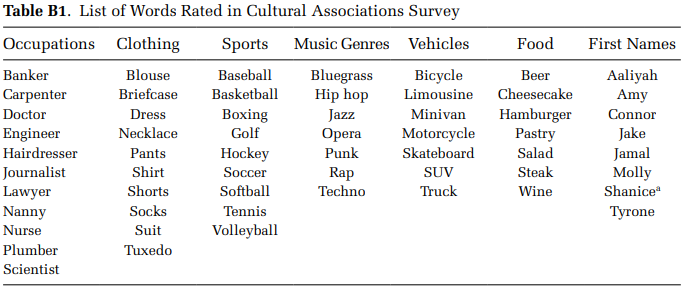
\includegraphics[scale = 0.6]{Images/kte_validation1.png}
    \end{figure}
\end{frame}
%%%%%%%%%%%%%%%%%%%%%%%%
\begin{frame}{KTE (2019): methods}{Validation}
\begin{figure}
    \centering
    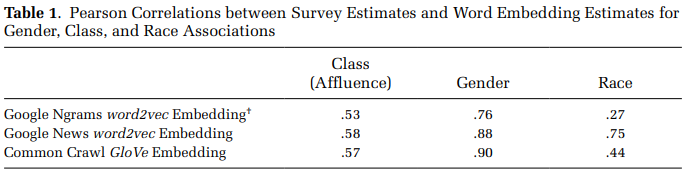
\includegraphics[scale = 0.6]{Images/kte_validation2.png}
    \end{figure}
\end{frame}
%%%%%%%%%%%%%%%%%%%%%%%%.
\begin{frame}{KTE (2019): methods}{Validation}
\begin{figure}
    \centering
    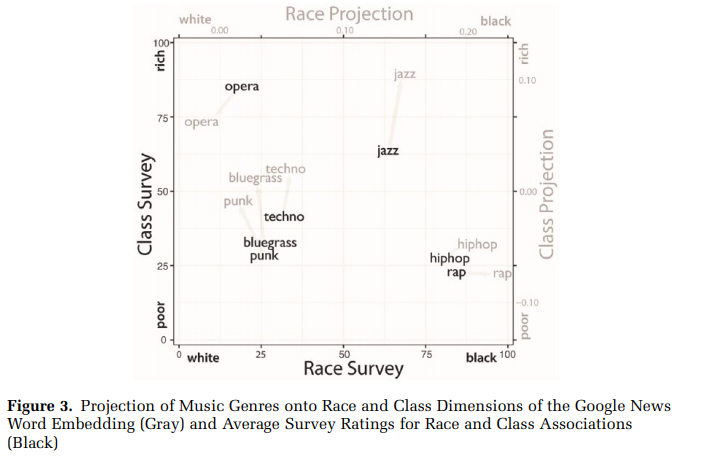
\includegraphics[scale = 0.6]{Images/kte_validation3.png}
    \end{figure}
\end{frame}
%%%%%%%%%%%%%%%%%%%%%%%%
\begin{frame}{KTE (2019): results}
\begin{figure}
    \centering
    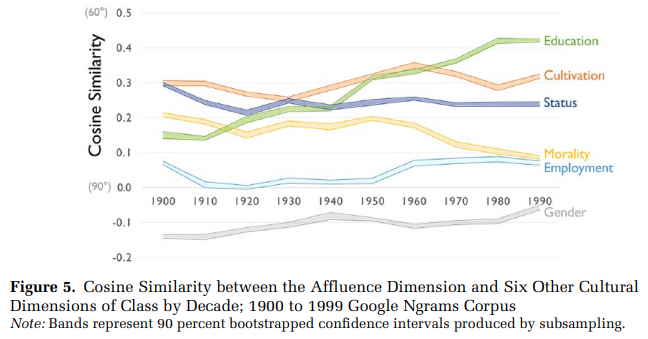
\includegraphics[scale = 0.5]{Images/kte_validation4.png}
    \end{figure}
\begin{itemize}
    \item Education has become more \textcolor{blue}{synonymous} with \textbf{affluence}
    \begin{itemize}
\vspace{6pt}
    \setlength{\itemsep}{0.6em}
        \item Crucial for a competitive labor market $\rightarrow$ \textbf{signaling}
        \item Mediated by cultivation: when controlled, negligible correlation
    \end{itemize}
\end{itemize}
\end{frame}
%%%%%%%%%%%%%%%%%%%%%%%%
\begin{frame}{KTE (2019): results}
\begin{figure}
    \centering
    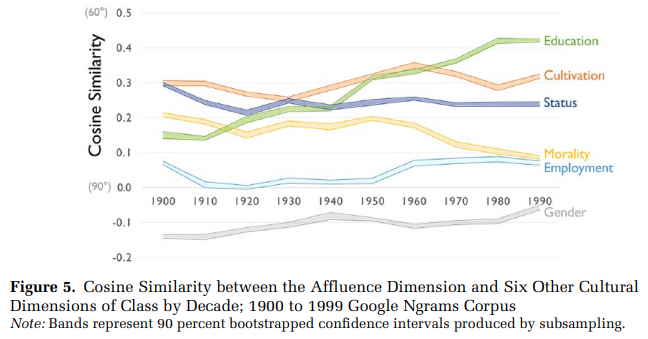
\includegraphics[scale = 0.5]{Images/kte_validation4.png}
    \end{figure}
\begin{itemize}
    \item Gender: \textcolor{blue}{positive} association between femininity and \textbf{affluence}
    \begin{itemize}
\vspace{6pt}
    \setlength{\itemsep}{0.6em}
        \item Veblen's idea of women as vessels for men's \textit{vicarious consumption}
        \item Words strongly projected include \textit{fragance, jewel, gem, perfume}
    \end{itemize}
\end{itemize}
\end{frame}
%%%%%%%%%%%%%%%%%%%%%%%%
\begin{frame}{KTE (2019): results}
\begin{figure}
    \centering
    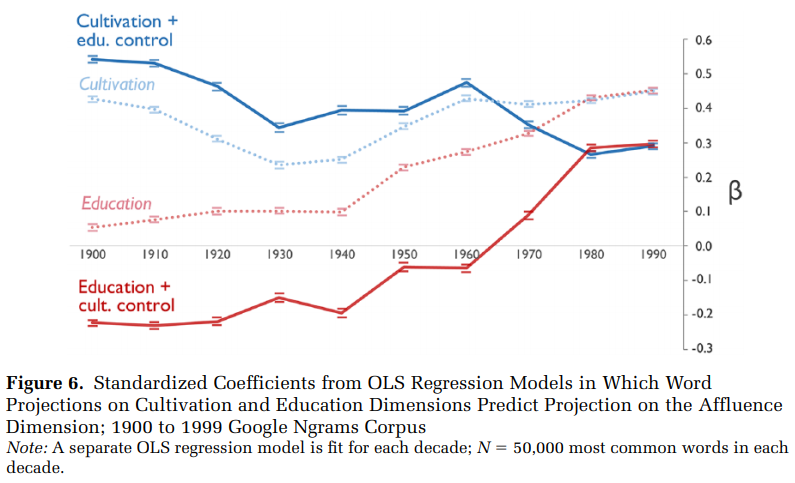
\includegraphics[scale = 0.5]{Images/kte_resultsOLS.png}
    \end{figure}
\end{frame}
%%%%%%%%%%%%%%%%%%%%%%%%
\end{document}
